\documentclass{beamer}
\mode<presentation>
% The Beamer class comes with a number of default slide themes
% which change the colors and layouts of slides. Below this is a list
% of all the themes, uncomment each in turn to see what they look like.
  %\usetheme{default}
  %\usetheme{AnnArbor}
  %\usetheme{Antibes}
  %\usetheme{Bergen}
  %\usetheme{Berkeley}
  %\usetheme{Berlin}
  %\usetheme{Boadilla}
  %\usetheme{CambridgeUS}
  %\usetheme{Copenhagen}
  %\usetheme{Darmstadt}
  %\usetheme{Dresden}
  %\usetheme{Frankfurt}
  %\usetheme{Goettingen}
  %\usetheme{Hannover}
  %\usetheme{Ilmenau}
  %\usetheme{JuanLesPins}
  %\usetheme{Luebeck}
  \usetheme{Madrid}
  %\usetheme{Malmoe}
  %\usetheme{Marburg}
  %\usetheme{Montpellier}
  %\usetheme{PaloAlto}
  %\usetheme{Pittsburgh}
  %\usetheme{Rochester}
  %\usetheme{Singapore}
  %\usetheme{Szeged}
  %\usetheme{Warsaw}

  % As well as themes, the Beamer class has a number of color themes
  % for any slide theme. Uncomment each of these in turn to see how it
  % changes the colors of your current slide theme.

  %\usecolortheme{albatross}
  %\usecolortheme{beaver}
  %\usecolortheme{beetle}
  %\usecolortheme{crane}
  %\usecolortheme{dolphin}
  %\usecolortheme{dove}
  %\usecolortheme{fly}
  %\usecolortheme{lily}
  %\usecolortheme{orchid}
  %\usecolortheme{rose}
  %\usecolortheme{seagull}
  %\usecolortheme{seahorse}
  %\usecolortheme{whale}
  %\usecolortheme{wolverine}
  %\setbeamertemplate{footline} % To remove the footer line in all slides uncomment this line
  %\setbeamertemplate{footline}[page number] % To replace the footer line in all slides with a simple slide count uncomment this line
  %\setbeamertemplate{navigation symbols}{} % To remove the navigation symbols from the bottom of all slides uncomment this line

  \usepackage{graphicx} % Allows including images
  \usepackage{amsmath,amsthm,amsfonts,mathtools,color,amssymb}
  \usepackage{bm}
  \usepackage{booktabs} % Allows the use of \toprule, \midrule and \bottomrule in tables

  \title[Research Update]{Spring research update} % The short title appears at the bottom of every slide, the full title is only on the title page

  \author{Emily Palmer} % Your name
  \institute[OSU] % Your institution as it will appear on the bottom of every slide, may be shorthand to save space
  {Oregon State University \\ % Your institution for the title page
    \medskip
    \textit{palmerem@oregonstate.edu} % Your email address
  }
  \date{\today} % Date, can be changed to a custom date

  \begin{document}

  \begin{frame}
  \titlepage % Print the title page as the first slide
  \end{frame}



%----------------------------------------------------------------------------------------
\begin{frame}
\frametitle{Approach}
\begin{itemize}
  %TODO
  \item Use Generalized estimating equations to estimate regression parameters and covariance parameters for microbiome relative abundances
  \item Assume the mean and variance follow those of the Dirichlet distribution
  \item Assume the correlation structure between ASVs in a sample depends both on compositionality and phylogenetic similarity
\end{itemize}
\end{frame}
%----------------------------------------------------------------------------------------

%----------------------------------------------------------------------------------------
\begin{frame}
\frametitle{Notation and setup}
\begin{itemize}
  \item Let $y_{ij}$ be the relative abundance of the $j$th ASV in the $i$th sample. $i = 1, \ldots , n, j = 1, \ldots , p$
  \item Assume that $E(y_{ij})  = \mu_{ij} = \frac{\alpha_{ij}}{\alpha_{i0}}$
  where $\alpha_{i0} = \sum_{j = 1}^p \alpha_{i0}$.

  and $\alpha_i$ are the parameters of if
  $\mathbf{y}_i \sim \text{Dirichlet}(\alpha_1, \ldots , \alpha_p)$

  \item Link function: Link covarites to $\alpha$'s:
  $$\log(\alpha_{ij}) = \mathbf{x_i}^T\boldsymbol\beta_j$$
  % and
  % $$\alpha_{ij} = e^{\mathbf{x_i}^T\boldsymbol\beta_j}$$
\end{itemize}
\end{frame}
%----------------------------------------------------------------------------------------


%----------------------------------------------------------------------------------------
\begin{frame}
\frametitle{Compositional Dirichlet Correlation}
\begin{itemize}
  \item Since ASVs are in relative abundances, we believe there is a negative correlation arising from compositionality.
  \item Dirichlet correlation:
  for $j \neq k$
  \[ R_{i,D} = Cor(y_{ij}, y_{ik})  = - \frac{\alpha_{ij}\alpha_{ik}}{\alpha_{i0}^2(\alpha_{i0} + 1)\sqrt{V(y_{ij})V(y_{ik})}} \]
  \[ V_{ij} = \frac{\alpha_{ij}(\alpha_{i0} - \alpha_{ij})}{\alpha_{i0}^2(\alpha_{i0} + 1)} \]
\end{itemize}
\end{frame}
%----------------------------------------------------------------------------------------
%----------------------------------------------------------------------------------------
\begin{frame}
\frametitle{GEE Algorithm}
\begin{itemize}
  \item Need to estimate $\beta, \rho, \omega$
  \item Fisher scoring algorithm
  \item Alternate by using current values of $\rho $ and $\omega$ (And thus $R_i$) to find $\beta$ and using current value of $\beta$ (and thus $\alpha$, $\epsilon$) to calculate $\rho, \omega$
\end{itemize}
\end{frame}
%----------------------------------------------------------------------------------------


\begin{frame}
\frametitle{Evolutionary Trait Correlation}
\begin{itemize}
  \item We borrow the idea of the evolutionary trait model (Martins and Hansen 1997) used in microbiome data models (Xiao et al 2018)
  \item From a phylogenetic tree, create matrix $\mathbf{D}$ where $d_{ij}$ is the distance between ASV $i$ and $j$.
  \item Use patristic distance - length of the shortest path.
  \item Correlation between ASV $j$ and $k$ is
  $$R_{i,ETM} = Cor(y_{ij}, y_{ik})  = e^{-2\rho d_{jk}}$$ Where $\rho > 0$ and needs to be estimated.
\item If $\rho$ is small, $R_{ijk}$ is close to 1 indicating high correlation. If $\rho$ is large, indicates no correlation.
  \item Interpretation of $\rho$: depth of the phylogenetic tree where groups are formed.
\end{itemize}
\end{frame}


%----------------------------------------------------------------------------------------
\begin{frame}
\frametitle{Working Correlation matrix}
\begin{itemize}
  \item Use weighted sum of Dirichlet compositional correlation and evolutionary trait model correlation
  \[R = \omega R_{Dir} + (1-\omega)R_{ETM} \]
\end{itemize}
\end{frame}
%----------------------------------------------------------------------------------------

%----------------------------------------------------------------------------------------
\begin{frame}
\frametitle{GEE Equations}
The GEE equations are

\begin{align*}
  \sum_{i = 1}^n  \left(\frac{\partial  \boldsymbol\mu_i }{\partial \boldsymbol\beta }\right)^t\mathbf{V}_i^{-1}(\mathbf{Y_i} - \boldsymbol\mu_i) = 0
\end{align*}

\begin{itemize}
  \item Where $ V_i = \frac{1}{\phi} A_i^{\tfrac{1}{2}}R_iA_i^{\tfrac{1}{2}}$

  \item $A_i = diag(V(Y_{ij}))$


  \item $ \left(\frac{\partial  \boldsymbol\mu_i }{\partial \boldsymbol\beta }\right)^t  = \frac{1}{\alpha_{i0}^2} (\alpha_{i0} \text{diag}(\alpha_i) - \alpha_i \alpha_i^t)  \otimes X_i$


\end{itemize}



\end{frame}
%----------------------------------------------------------------------------------------

%----------------------------------------------------------------------------------------
\begin{frame}
\frametitle{GEE Algorithm - $\rho, \omega, \phi$ step}

GEE algorithm goes between steps for estimating $\rho, \omega, $ and $\phi$ and step for estimating $\beta$.

\begin{itemize}
  \item $e_{ij} = y_{ij} - \mu_{ij}$
  \item $\phi = \left(\frac{1}{n*p - (p*q - 1)}\sum_{i = 1}^n \sum_{j = 1}^p e_{ij}^2 \right) ^{-1}$
  \item $\omega, \rho$ minimize
  \[ \sum (\phi e_{ij}e_{ik} - [ \omega R_{ijk,D} + (1 - \omega) e^{-2 \rho D_{jk}}])^2  \]
  suject to $0 \leq \omega \leq 1, \rho > 0$
  \item Given $\rho, \omega,$ working correlation $R$ is specified.
\end{itemize}

\end{frame}
%----------------------------------------------------------------------------------------



%----------------------------------------------------------------------------------------
\begin{frame}
\frametitle{GEE Calculate $\omega, \rho$}
\begin{itemize}
  \item Use "L-BFGS-B" algorithm (Byrd et. al. (1995))
  \item Option in \texttt{optim()} that allows bounds to be specified $0 \leq \omega \leq 1, \rho > 0$
  \item This uses a limited-memory modification of the BFGS quasi-Newton method.
\end{itemize}
\end{frame}
%----------------------------------------------------------------------------------------

%----------------------------------------------------------------------------------------
\begin{frame}
\frametitle{GEE Algorithm - $\beta$ step}

\[G =  \sum_{i = 1}^n  \left(\frac{\partial  \boldsymbol\mu_i }{\partial \boldsymbol\beta }\right)^t\mathbf{V}_i^{-1}(\mathbf{Y_i} - \boldsymbol\mu_i)\]
\[H = - \sum_{i=1}^n \left(\frac{\partial  \boldsymbol\mu_i }{\partial \boldsymbol\beta }\right)^t V_i ^{-1} \frac{\partial  \boldsymbol\mu_i }{\partial \boldsymbol\beta } + \lambda I \]

\[\hat\beta^{(s +1)} = \hat\beta^{(s)} - \gamma H ^{-1} G \]

% Where $0 < \gamma < 1$ is found using a line search

\end{frame}
%----------------------------------------------------------------------------------------

%----------------------------------------------------------------------------------------
\begin{frame}
\frametitle{$\beta$-step considerations}
\begin{itemize}
  \item $H$ is or is close to singular. Add a small diagonal constant. $\lambda$
  (depending on eigenvalues of H)
  \item Appears that steps are too large, which leads to quick divergence and infinite estimates.
  \item Currently implementing a line search algorithm. Check sum of squared GEE values and iteratively set $\gamma^{k+1} = \frac{1}{2}\gamma^k$ until there is a reduction.
  %TODO
\end{itemize}
\end{frame}
%----------------------------------------------------------------------------------------

%----------------------------------------------------------------------------------------
\begin{frame}
\frametitle{Real data - Zebrafish data}
\begin{itemize}
  \item
	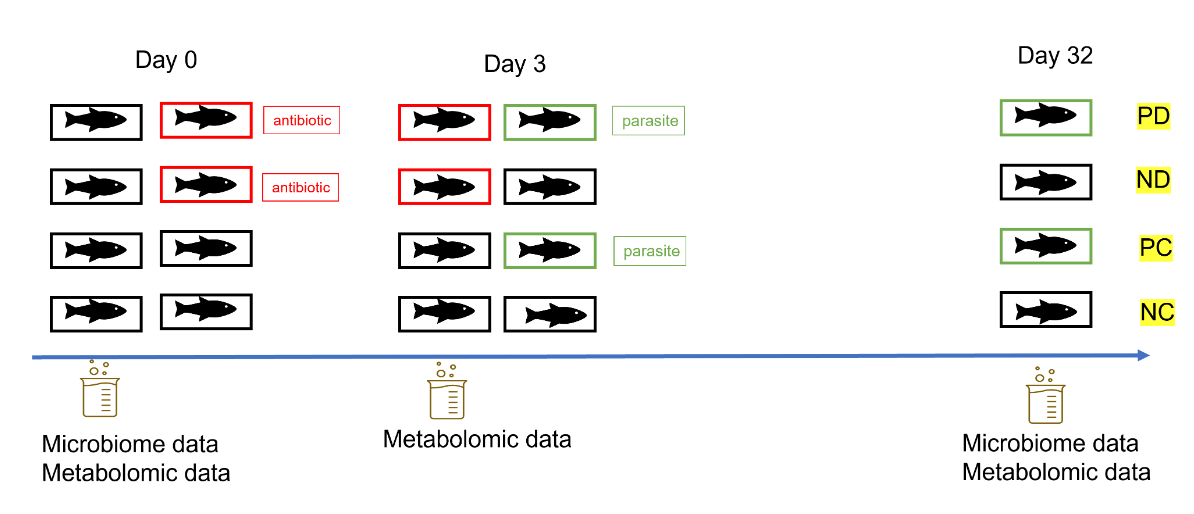
\includegraphics[width=0.65\textwidth]{img/2022_April_11_Research_Update-f2887a67.png}
  \item Use only day 32
  \item Filter taxa to only include if present in 30\% of samples
  \item Use covariate of parasite/no parasite introduced
  \item Using 68 samples and 39 taxa.
  \item Initially using data to get algorithm up and running, now transitioning to looking for results.
\end{itemize}
\end{frame}
%---------------------------------------------------------
%----------------------------------------------------------------------------------------
\begin{frame}
\frametitle{Real Data - Results}
\begin{itemize}
  \item $\omega  = 0.79$
  \item $\rho = 4.4$
  \item 80\% of estimated correlation is due to the compositional structure, 20\% is from phylogenetic correlation,
  \item $\beta = $
  \item Sandwhich etimator
  \item Include heatmap of correlations?

  \[ (X^tX)^{-1} [\sum_i(y_i - \hat\mu_i)(y_i - \hat\mu_i)^tX_i](X^tX)^{-1}\]
\end{itemize}
\end{frame}
%----------------------------------------------------------------------------------------



%----------------------------------------------------------------------------------------
\begin{frame}
\frametitle{Current challenges}
\begin{itemize}
  \item Currently working on various numerical challenges:
  \item When data are not filtered so strictly (eg 10\% or 20\%), algorithm would not converge or was unstable. A less strict filter results in both a larger percent zero data but also an increase in parameters.
  \item Belieive to be due to close to singular hessian matrix.
  \item Stability of estimates of $\rho, \omega$ sensitive to initial starting values of each step.
\end{itemize}
\end{frame}
%----------------------------------------------------------------------------------------
%----------------------------------------------------------------------------------------
\begin{frame}
\frametitle{Questions - Phylogenetic analysis}
\begin{itemize}
  \item Currently analysis is done on the ASV level.
  \item Could we perform analysis on the Genus level?
  \item How would we consolidate the phylogenetic tree (and calculate distances) at the Genus level?
  \item Is this reasonable/appropriate?
\end{itemize}
\end{frame}
%----------------------------------------------------------------------------------------

%----------------------------------------------------------------------------------------
\begin{frame}
\frametitle{Questions \& next steps}
\begin{enumerate}
  \item What are covariates or groups of covariates that are more of interest?
  \item How to calculating significance? Can use sandwhich estimator and asymptotic normality. Permutations?
\end{enumerate}
\end{frame}
%----------------------------------------------------------------------------------------

%----------------------------------------------------------------------------------------
\begin{frame}

Thank you!

\end{frame}
%----------------------------------------------------------------------------------------





  \end{document}
